\newpage
\section{Vorbereitungsfragen}
\subsection{1}
\begin{figure}[H]
    \centering
    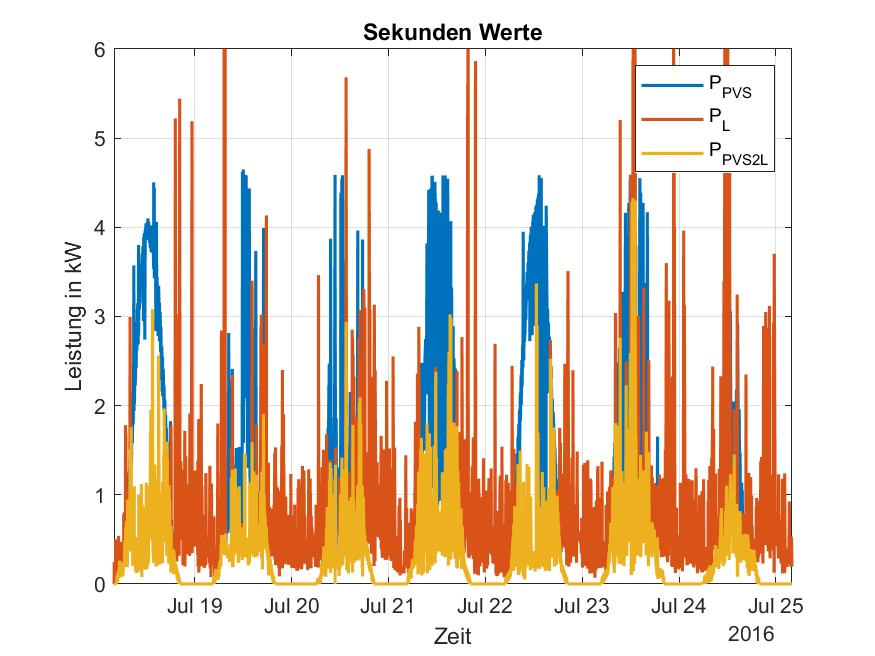
\includegraphics[width=\textwidth]{Abbildungen/plot.jpg}
    \caption{Beschreibung des Plots}
    \label{fig:plot3062023}
\end{figure}
\begin{figure}[H]
    \centering
    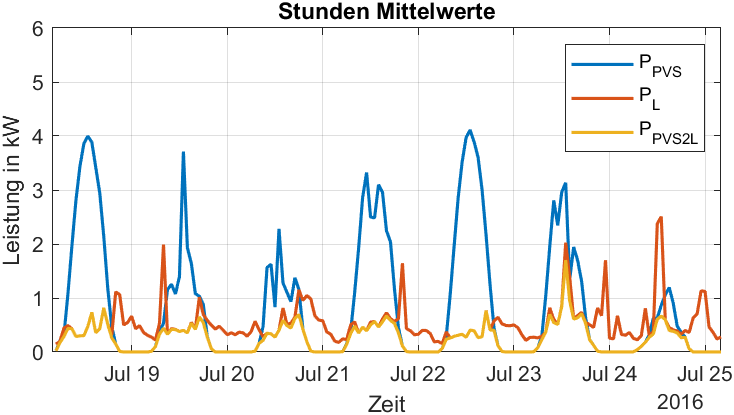
\includegraphics[width=\textwidth]{Abbildungen/aufgabe1_plot2.png}
    \caption{}
    \label{fig:plot1_2_3062023}
\end{figure}
\subsection{Ermitteln Sie über den gesamten Messzeitraum die Energiesummen EPVS, EL und EPVS2L der
Leistungsvariablen PPVS, PL und PPVS2L (Angabe in kWh).}
Die zu ermittelnden Energiesummen lauten wie folgt:
\\

$E.E_pvs = sum(ts.Ppvs/1000)/3600=149,96kWh;\\
E.E_l = sum(ts.Pl/1000)/3600=89,08kWh;\\
E.E_pvs2l = sum(Ppvs2l/1000)/3600=41,52kWh;$\\

\subsection{Berechnung der Differenzleistung}
\begin{figure}[H]
    \centering
    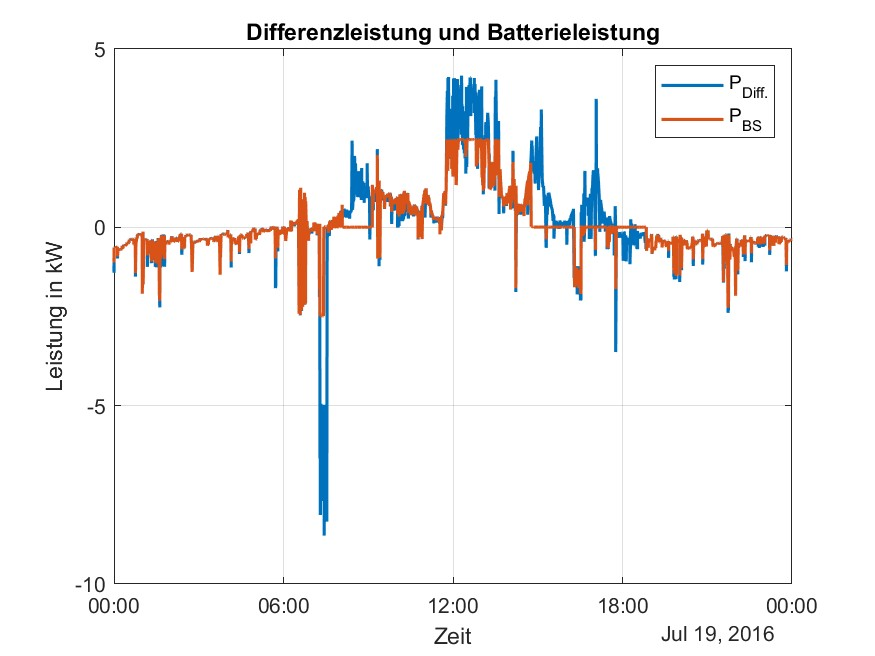
\includegraphics[width=\textwidth]{Abbildungen/plot_vorbereitungsfrage3.jpg}
    \caption{Differenzleistung und Batterieleistung im Vergleich}
    \label{fig:plot3062023_2}
\end{figure}
In \autoref{fig:plot3062023_2} ist die Differenz- sowie Batteriesystemleistung zu sehen. 
Die Batteriesystemleistung dient als Richtschnur, um festzustellen, ob es zu einem bestimmten Zeitpunkt geladen oder entladen wird. 
Eine positive Differenzleistung deutet auf einen Überschuss an Energie hin, wodurch das Batteriesystem aufgeladen werden kann, falls es nicht bereits vollständig geladen ist. Im Gegensatz dazu signalisiert eine negative Differenzleistung einen Energiemangel, der in erster Linie durch das Batteriesystem ausgeglichen werden sollte.
Dabei ist zu erkennen, dass die Differenzleistung größer ist als die Batterieleistung. 
Dies liegt daran, dass der Batteriespiecher nur eine endliche Menge an Leistung auf und abgeben kann.

\subsection{Funktionsweise des cumsum Befehls}
\begin{figure}[H]
    \centering
    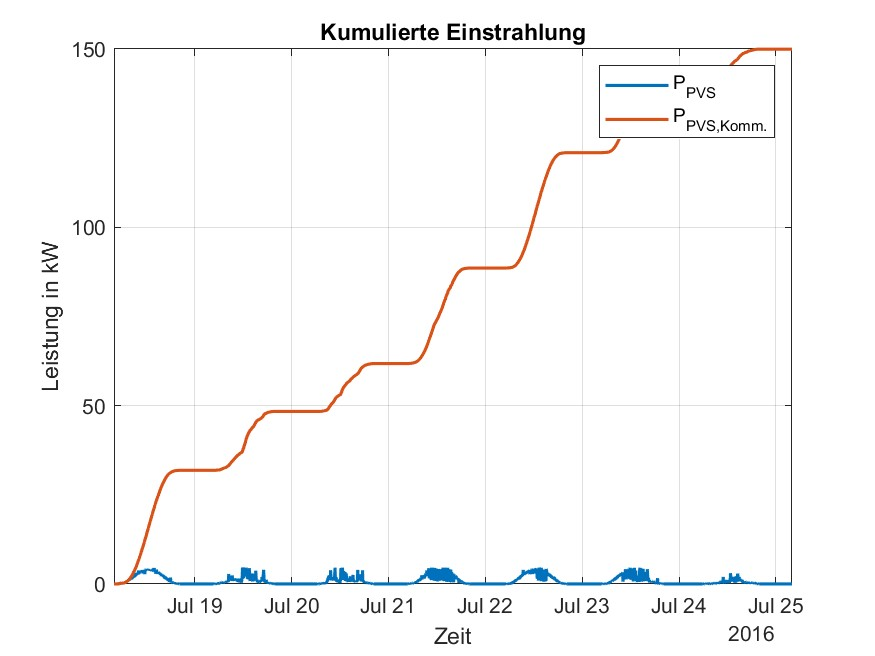
\includegraphics[width=\textwidth]{Abbildungen/plot_vorbereitungsfrage4.jpg}
    \caption{Anschauliche Darstellung des cumsum Befehls}
    \label{fig:plot43062023}
\end{figure}
Der MATLAB-Befehl cumsum steht für cumulative sum und wird verwendet, um die kumulative Summe eines Vektors oder einer Matrix zu berechnen. 
Also statt die gesammte Summe zu berechnen, werden mit cumsum auch alle zwischen Summen gespeichert. In \autoref{fig:plot43062023} ist zu sehen, wie mit Hilfe des Befehls die Leistungen kummuliert werden und man eine Aussage über die kummulierte Einstrahlung erhält.